\documentclass{article}

%
% 引入模板的style文件
%
\usepackage{homework}


%
% 封面
%

\title{
	
\includegraphics[scale = 0.45]{logo.jpg}\\
    \vspace{1in}
    \textmd{\textbf{XXX课程\ }}\\
   \textmd{\textbf{\hmwkSubTitle}}\\
    %\normalsize\vspace{0.1in}\small{\date{2022年5月15日} }\\
    \vspace{0.1in}\large{\textit{\hmwkClassInstructor\ }}\\
            \vspace{3in}
    \hmwMajor{}\\
    \hmwNumber{}\\
    \hmwkAuthorName{}\\
}



\date{\today}

\renewcommand{\part}[1]{\textbf{\large Part \Alph{partCounter}}\stepcounter{partCounter}\\}


%
% 正文部分
%
\begin{document}

\maketitle


%\include{chapters/ch01}
%\include{chapters/ch02}
%\include{chapters/ch03}
%\include{chapters/ch04}
%\include{chapters/ch05}


\pagebreak




\begin{homeworkProblem}
简述$QCD$渐进自由性质及与其他几种相互作用力间的区别。
	
	
	
\textbf{Solution}


由重整化群方程可知，经重整化后$QCD$满足演化方程($DGLAP$)如下
\[
\begin{split}
\frac{\partial f\left( x,\mu ^2 \right)}{\partial \ln \mu}=\frac{{\alpha ^2}_s}{2\pi}\int_x^1{\frac{dz}{z}}\sum_i{f_{i/X}}\left( \frac{x}{z},\mu ^2 \right) P_{ij}\left( z \right) 
\end{split}
\]	
其中$\mu$为能标，$f_{i/X}$为部分子$X$中动量$i$数量，$f\left( x,\mu ^2 \right)$为重整化后的场算符，于此处取couppling constant 为研究对象，考虑leading order 重整化得
\[
\begin{split}
Z_g&=1-\frac{{g_0}^2}{16\pi ^2}\left( \frac{11}{6}N_c-\frac{1}{3}N_f \right)\frac{1}{\epsilon},\\
\Rightarrow \beta(\mu^2)&=\mu \frac{\partial g_0}{\partial \mu} =-\frac{{g_0}^3}{8\pi ^2}\left( \frac{11}{6}N_c-\frac{1}{3}N_f \right) .
\end{split}
\]
不妨取研究能标为$g(\mu_R^2)$，重整化能标为$g(Q^2)$，$(\mu_R^2>Q^2)$，带入$\beta$函数可得
\[
\begin{split}
g\left( {\mu ^2}_R \right) =\frac{g\left( Q^2 \right)}{1+\frac{1}{8\pi ^2}\left( \frac{11}{6}N_c-\frac{2}{3}N_f \right) \ln \frac{{\mu ^2}_R}{Q^2}},
\end{split}
\]
带入$N_c=3,N_f=6$可得，在能标较高时耦合常数趋近于0，即在较高能标下自由度较低，较低能标下可近似认为处于核内自由态，该性质为强相互作用力独有，引力及电弱相互作用不具备该特性。
\end{homeworkProblem}	




\begin{homeworkProblem}
试区分电子与质子在弹性散射及非弹性散射间定义的区别	
	
\textbf{Solution}
\begin{enumerate}
	\item 弹性散射(ES)
	

电子与质子发生弹性散射时末态产物为电子与质子，无其他强子生成，其动量转移$Q^2=(p^{\prime}-p)^2$(p,$p^{\prime}$分别为电子初末态四动量)较小。

	\item 非弹性散射(DS)


电子与质子发生非弹性散射时末态产物为电子及强子，其动量转移$Q^2$较高。
	
	
	
\end{enumerate}
	
	
\end{homeworkProblem}	
\pagebreak



\begin{homeworkProblem}
试举例说明$QCD$色自由度为3的实验依据。
	
	
\textbf{Solution}	
考虑正反电子对湮灭产生强子或一对正反轻子对的过程，定义
\[
\begin{split}
R=\frac{\sigma (e^+e^-\rightarrow hardons)}{\sigma (e^+e^-\rightarrow leptons)},
\end{split}
\]	
由渐进自由可知，在刚好能产生$u,d,s$夸克时满足
\[
\begin{split}
R&\simeq N_c[(\frac{2}{3})^2+(-\frac{1}{3})^2+(-\frac{1}{3})^2]\\
&=\frac{2}{3}N_c.
\end{split}
\]
实验测量值$R\simeq 2$，进而可知色自由度为3。		
\end{homeworkProblem}	


\begin{homeworkProblem}
于$CM$系中试根据量子场论推导卢瑟福散射公式。

\textbf{Solution}	

取重核电荷量为$Ze$，质量为$M>>m_e$做费曼图如图所示，
\begin{figure}[H]  % 这里记得用[H]
\centering
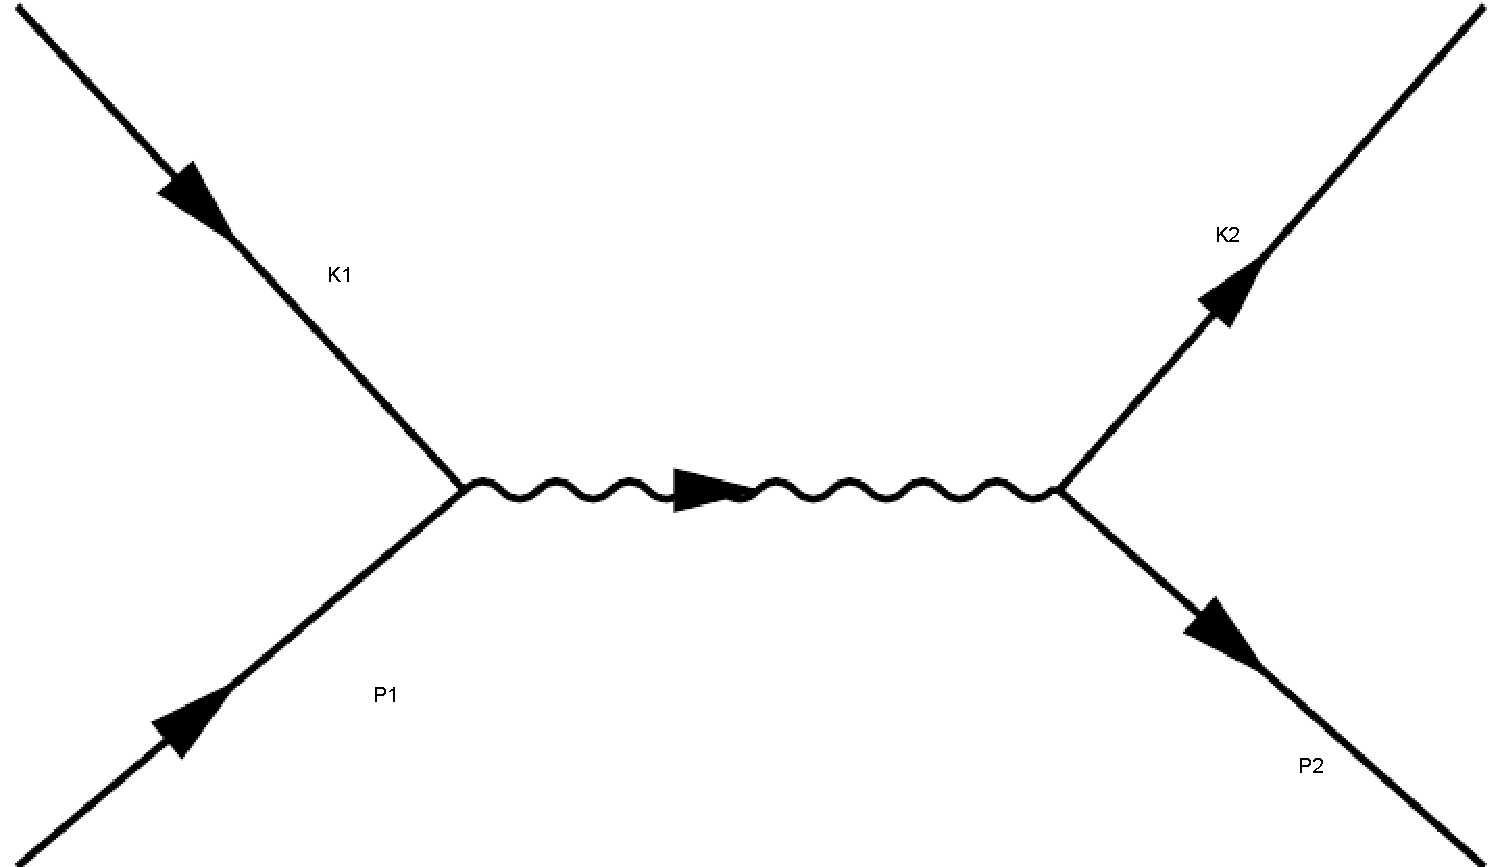
\includegraphics[width=0.7\linewidth]{3.pdf}
\caption{feynman diagram}
\label{fig:diagram}
\end{figure}	
可得
\[
\begin{split}
iM&=\bar{u}\left( p_2 \right) \left( -ie\gamma ^{\alpha} \right) u\left( p_1 \right) \frac{-ig_{\alpha \beta}}{q^2+i\epsilon}\bar{u}\left( p_2 \right) \left( -iZe\gamma ^{\beta} \right) u\left( p_2 \right) ,
\\
\Rightarrow \frac{1}{4}\sum_{spins}{|M|^2}&=\frac{8Z^2}{s^2}\left[ p_2\cdot k_2p_1\cdot k_1+p_2\cdot k_1p_1\cdot k_2-M^2p_1\cdot p_2-{m^2}_ek_1\cdot k_2+2{m^2}_eM^2 \right] 
\end{split}
\]
在$CM$系中有
\begin{figure}[H]  % 这里记得用[H]
	\centering
	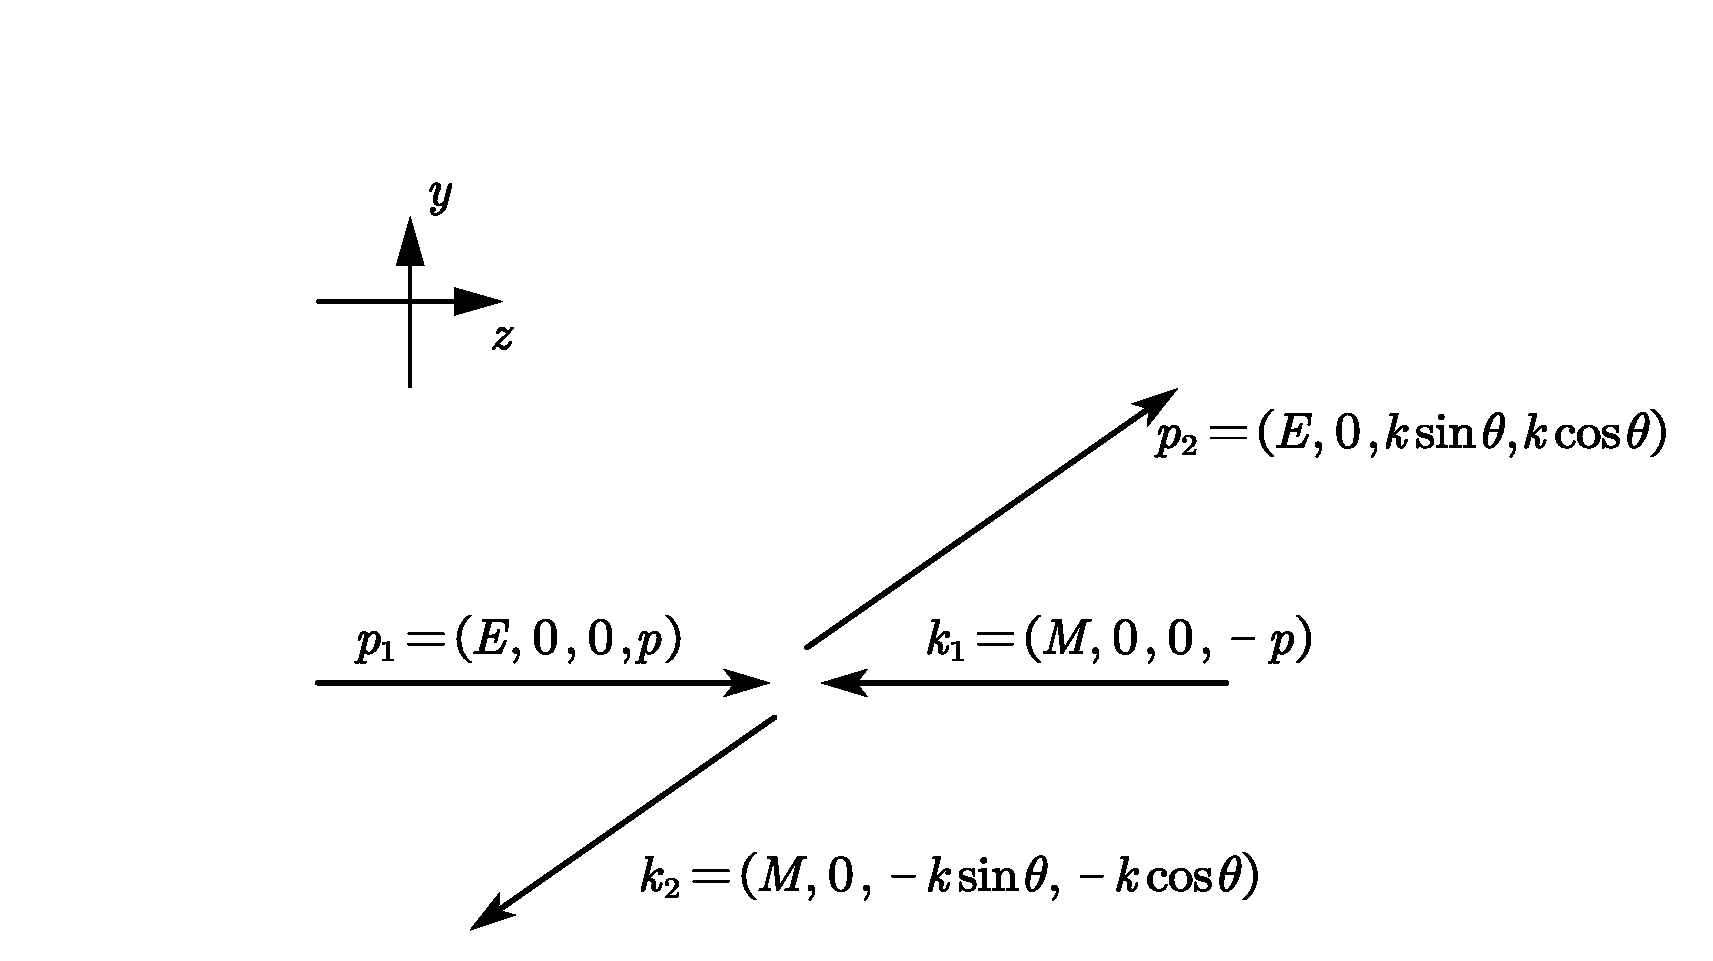
\includegraphics[width=0.7\linewidth]{7.pdf}
	\caption{feynman diagram}
	\label{fig:diagram}
\end{figure}
进而可得
\[
\begin{split}
\frac{1}{4}\sum_{spins}{|M|^2}&\simeq \frac{Z^2e^4\left( 1-|\vec{v}|^2\sin ^2\frac{\theta}{2} \right)}{|\vec{p}|^2|\vec{v}|^2\sin ^4\frac{\theta}{2}}M^2,
\\
\Rightarrow \left( \frac{d\sigma}{d\Omega} \right) _{CM}&=\frac{1}{2E\cdot 2M|\vec{v}|}\frac{1}{4}\sum_{spins}{|M|^2}
\\
&=\frac{Z^2{\alpha ^2}_s}{4|\vec{p}|^2|\vec{v}|^2\sin ^4\frac{\theta}{2}}\left( 1-|\vec{v}|^2\sin ^2\frac{\theta}{2} \right) .
\end{split}
\]
	
\end{homeworkProblem}	
	%\begin{figure}[H]  % 这里记得用[H]
		%\centering
		%\includegraphics[width=0.7\linewidth]{images/title/ucas-logo}
		%\caption{ucas-logo}
		%\label{fig:ucas-logo}
	%\end{figure}
	
%\[
%\begin{split}
%e_{u}=8.4\%,e_{s}=0.006\%,
%\end{split}
%\]	


%\begin{homeworkProblem}
%代码的示例：\\
	
%\begin{lstlisting}[language = HTML, numbers=left, 
%numberstyle=\tiny,keywordstyle=\color{blue!70},
%commentstyle=\color{red!50!green!50!blue!50},frame=shadowbox,
%rulesepcolor=\color{red!20!green!20!blue!20},basicstyle=\ttfamily]

%scheme:[//[user[:password]@]host[:port]][/path][?query][#fragment]


%\end{lstlisting}
	
	
%\end{homeworkProblem}

\end{document}
